\chapter{Compilation}

Before we start writing our own language, it is important to understand
how a compiler does its translation work.

All quality software is made in modules. Each module is focused on one
task. The inputs and outputs to it are clearly defined. If we reject
the design of a component, we can replace it. So long as the inputs and
outputs are the same, none of the other modules need alterations. Compilers
are modular.

To deduce what the compiler modules should be, think about the work to
be done. At the beginning there is a source file. We need to read that
text. This reading happens one character at a time, because many
of the things we care about are only one character, like a plus sign.

From the raw stream of characters, the next step forms tokens. These
are the basic elements of a program like a keyword, a brace, a number, or
one of those plus signs. The module that forms the tokens is called
the scanner, the tokenizer, or the lexer. That last term comes from
the longer name of this process: lexical analysis. Always remember
that the tokens are formed first. Nothing that happens further downstream
can adjust how the lexer formed the tokens.\footnote{There are other
parsing schemes where this is not the case, notably recursive descent
parsing favored in Perl and Raku. We won't go into that here.}

Given the token stream, the parser attempts to recognize the language
based on its gramamr. When that works, it builds an abstract syntax
tree (AST) which represents the particular program in a data structure.

With an AST you can immediately interpret the language, which is what we
will mainly do. You can also build a secondary tree (or directed graph).
Such a tree allows you to do two things: (1) further analize the program
for semantic errors, (2) optimize the program, which is usually to make
it run faster and/or use less memory.

Semantic analysis and optimization are optional additional modules in the
chain. You can have several of each. All of those take and produce
the same internal representation. That allows us to mix and match them.

Finally, the last module emits a target language. Notice that this
"finally" might in fact kick off further processing. For instance, if you
make a PDF, you would still need a viewer to render it. Or, in a setup
like gcc, you would emit assembly, then immediately assemble and link
the result into an executable. In that case, assembling and linking would
be additional steps.

This is what the whole process looks like from source to target.

\begin{figure}
\centering
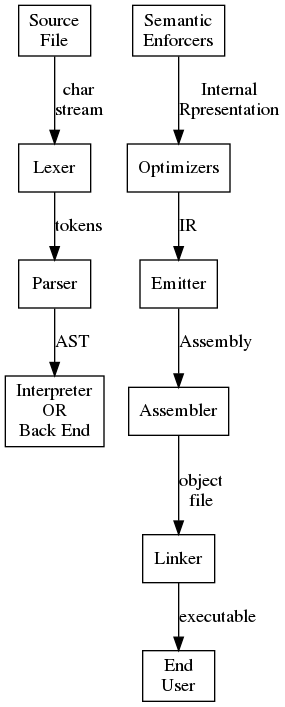
\includegraphics[scale=0.70]{compilationsteps.png}
\end{figure}

I've divided this at a logical point partly for screen layout,
but also to show the front and back halves of the chain.

The parser makes the AST. Something walks that. To start, we will
walk that with an interpreter and avoid the back half entirely.
If you move on to the back, you need the visitor to make an internal
representation (IR). This is either another tree or a directed graph.
That is what the semantic analyzers, optimizers, and emitters use.

Again, after you emit the target language compilation is finished,
but the process might continue. Perhaps you need to bundle the result
into a form that can be delivered economically to a browser, or your
target was assembly that needs to be assebled and linked. We won't
have any concern for those final steps. Once the target is reached,
we will leave the rest of the tools to others.
